The behavior of the time varying electromagnetic field in the free space is governed by the microscopic variant of Maxwell equations,
\begin{equation}
\label{3.1.1.1}
\nabla \cdot \vec{E} = \frac{\rho}{\varepsilon_{0}}, \qquad \nabla \cdot \vec{B} = 0
\end{equation}
\begin{equation}
\label{3.1.1.2}
\nabla \times \vec{E} = - \diffp{\vec{B}}{t}, \qquad \nabla \times \vec{B} = \mu_{0} \vec{J} + \frac{1}{c^{2}} \diffp{\vec{E}}{t},
\end{equation}
where $ \rho\left(\vec{x}, t \right) $ is charge density and $ \vec{J}\left(\vec{x}, t \right) $ current density.

To make the simulation possible, PIC method solves field equations only at certain points of the computational domain and time levels. Therefore, it is necessary to perform the discretization of the spatial coordinates $ \vec{x} \rightarrow x_{i, j, k} $ where $ (i,j,k) \in \mathbb{N}^{3} $ are grid indices and the time coordinate $ t \rightarrow t^{\,n} $, where $ n \in \mathbb{N} $ is the time level index. Solution is outlined here for a three-dimensional equidistant rectangular grid, thus $ x_{i, j, k} = \left(i \Delta x, j \Delta y, k \Delta z\right) $ where $ \Delta x, \Delta y, \Delta z $ are the spatial steps in each direction and $ t^{\,n} = n\Delta t $ where $ \Delta t $ is the time step.

Typical method to solve Maxwell equations in PIC codes is finite-difference time-domain (FDTD), because it is arguably the simplest technique in terms of the implementation. The vector components of the fields $ \vec{E} $ and $ \vec{B} $ are spatially staggered about rectangular unit cells of a Cartesian computational grid,
\begin{equation}
\label{3.1.1.4}
\vec{E}\left(\vec{x}, t \right) \rightarrow \left[\left(E_{x}\right)^{n}_{i,\: j + 1/2,\: k + 1/2}, \left(E_{y}\right)^{n}_{i + 1/2,\: j,\: k + 1/2}, \left(E_{z}\right)^{n}_{i + 1/2,\: j + 1/2,\: k} \right],
\end{equation}
\begin{equation}
\label{3.1.1.5}
\vec{B}\left(\vec{x}, t \right) \rightarrow \left[\left(B_{x}\right)^{n}_{i + 1/2,\: j,\: k}, \left(B_{y}\right)^{n}_{i,\: j + 1/2,\: k}, \left(B_{z}\right)^{n}_{i,\: j,\: k + 1/2} \right].
\end{equation}
This scheme, which has proven to be very robust, is now known as a Yee lattice \cite{yee}. The illustration of a standard Cartesian Yee cell used for FDTD is shown in Figure \ref{3.1.1.14}. Components of the current density $ \vec{J} $ are defined in the same way as the components of $ \vec{E} $ , charge density is defined in the middle of the cell. For marching in time a leap-frog scheme is used, thus discretized Maxwell equations (\ref{3.1.1.1}), (\ref{3.1.1.2}) have the following form,
\begin{equation}
\label{3.1.1.6}
\nabla^{+} \cdot \vec{E}^{\:n} = \frac{\rho^{\:n}}{\varepsilon_0}, \quad \nabla^{-} \cdot \vec{B}^{\:n + 1/2} = 0.
\end{equation}
\begin{equation}
\label{3.1.1.7}
\frac{\vec{B}^{\:n + 1/2} - \vec{B}^{\:n - 1/2}}{\Delta t} = -\nabla^{-} \times \vec{E}^{\:n}, \quad \frac{1}{c^{2}} \frac{\vec{E}^{\:n + 1} - \vec{E}^{\:n}}{\Delta t} = \nabla^{+} \times \vec{B}^{\:n + 1/2} - \mu_{0} \vec{J}^{\:n + 1/2},
\end{equation}
Notice that FDTD method achieve second-order accuracy in both, space and time. Discrete operators $ \left(\nabla^{+}\right) $ and $ \left(\nabla^{-}\right) $ act on a scalar field $ f_{i, j, k} $,
\begin{equation}
\label{3.1.1.8}
\nabla^{+} f_{i,\: j,\: k} = \left(\frac{f_{i + 1,\: j,\: k} - f_{i,\: j,\: k}}{\Delta x}, \frac{f_{i,\: j + 1,\: k} - f_{i,\: j,\: k}}{\Delta y}, \frac{f_{i,\: j,\: k + 1} - f_{i,\: j,\: k}}{\Delta z} \right), 
\end{equation}
\begin{equation}
\label{3.1.1.9}
\nabla^{-} f_{i,\: j,\: k} = \left(\frac{f_{i,\: j,\: k} - f_{i - 1,\: j,\: k}}{\Delta x}, \frac{f_{i,\: j,\: k} - f_{i,\: j - 1,\: k}}{\Delta y}, \frac{f_{i,\: j,\: k} - f_{i,\: j,\: k - 1}}{\Delta z} \right).
\end{equation}
These operators have the following properties,
\begin{equation}
\label{3.1.1.10}
\nabla^{-} \cdot \nabla^{-} \times = \nabla^{+} \cdot \nabla^{+} \times = 0, \qquad \nabla^{-} \cdot \nabla^{+} = \nabla^{+} \cdot \nabla^{-} = \Delta.
\end{equation}
Symbol $ \Delta $ stands for the discrete Laplace operator in central differences,
\begin{equation}
\label{3.1.1.11}
\Delta f_{i, j, k} = \frac{f_{i - 1, j, k} + 2 f_{i, j, k} + f_{i + 1, j, k}}{\Delta x^{2}} + \frac{f_{i, j - 1, k} + 2 f_{i, j, k} + f_{i, j + 1, k}}{\Delta y^{2}} + \frac{f_{i, j, k - 1} + 2 f_{i, j, k} + f_{i, j, k + 1}}{\Delta z^{2}}.
\end{equation}
\begin{figure}[h!]
\centering
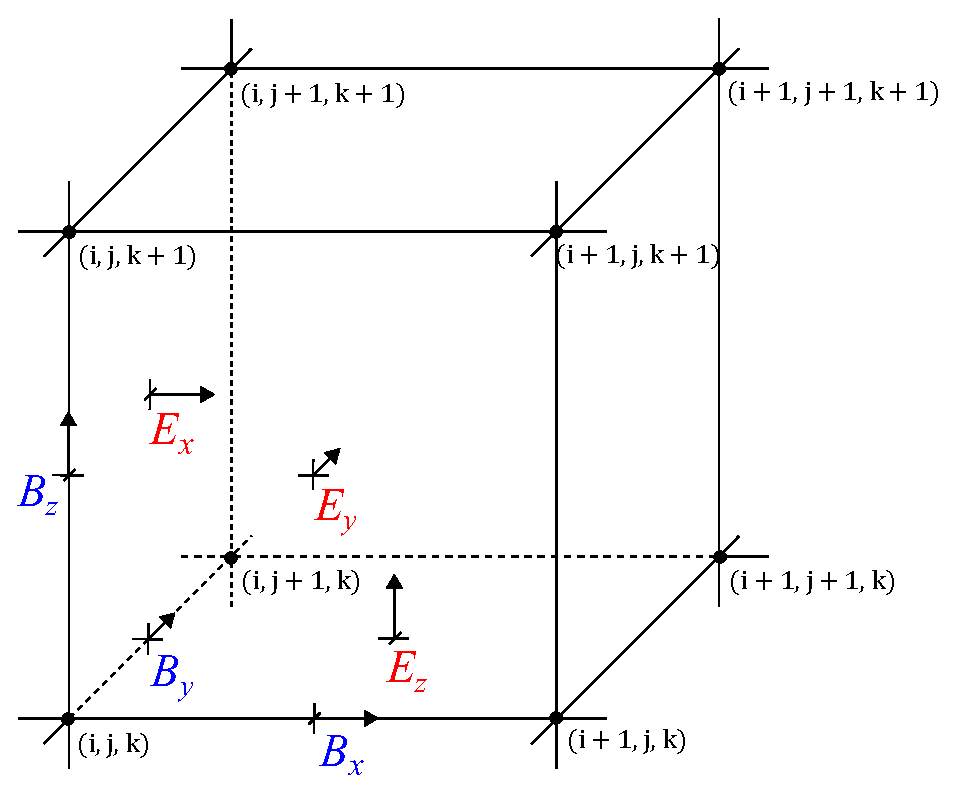
\includegraphics[width=0.4\paperwidth]{./img/YEE/yee.eps}
\caption{Standard Cartesian Yee cell used for FDTD method}
\label{3.1.1.14}
\end{figure}

Before trying to find the solution of Maxwell equations, one have to realize that this system of equations is not independent. In the three-dimensional case, there are eight first-order differential equations, but only six unknown vector components. Acting on the first and second of the equations (\ref{3.1.1.7}) by operators $ \left(\nabla^{-}\cdot\right) $ and $ \left(\nabla^{+}\cdot\right) $, respectively, one obtains
\begin{equation}
\label{3.1.1.12}
\frac{\nabla^{-} \cdot \vec{B}^{\:n + 1/2} - \nabla^{-} \cdot \vec{B}^{\:n - 1/2}}{\Delta t} = 0,
\end{equation}
\begin{equation}
\label{3.1.1.13}
\frac{\rho^{\:n + 1} - \rho^{\:n}}{\Delta t} + \nabla^{+} \cdot \vec{J}^{\:n + 1/2} = 0.
\end{equation}
It means that it is possible to solve only equations (\ref{3.1.1.7}), while the divergence equations (\ref{3.1.1.6}) can be considered as initial conditions. In this case, the continuity equation in finite differences (\ref{3.1.1.13}) have to be fulfilled.